%!TEX encoding = UTF-8 Unicode
%!TEX program = xelatex

\documentclass[bachelor]{ustcthesis}
% bachelor|master|doctor
\usepackage{ustcextra}
\usepackage{pdfpages}
\usepackage{float}
\restylefloat{table}
\graphicspath{{figures/}}
%\bibliographystyle{ustcauthoryear}
\bibliographystyle{ustcnumerical}

\title{基于卷积神经网络的电影评分预测}
\author{姚凯}
\major{计算机科学与技术专业}
\advisor{曹涌\ 主管研究员\ ,金培权\ 副教授}
\submitdate{二〇一七年五月}
%\secrettext{机密\quad 小于等于20年}   % 内部|秘密|机密,注释本行则不保密
\depart{计算机科学与技术系}

\entitle{Convolutional Neural networks based movie rates prediction}
\enauthor{Kai Yao}
\enmajor{Computer Science and Technology}
\enadvisor{Yohn Cao, Peiquan Jin}
\ensubmitdate{May, 2017}
%\ensecrettext{Confidential\quad Less than or equal to 20 years}  % Internal|Secret|Confidential

\begin{document}

%\maketitle
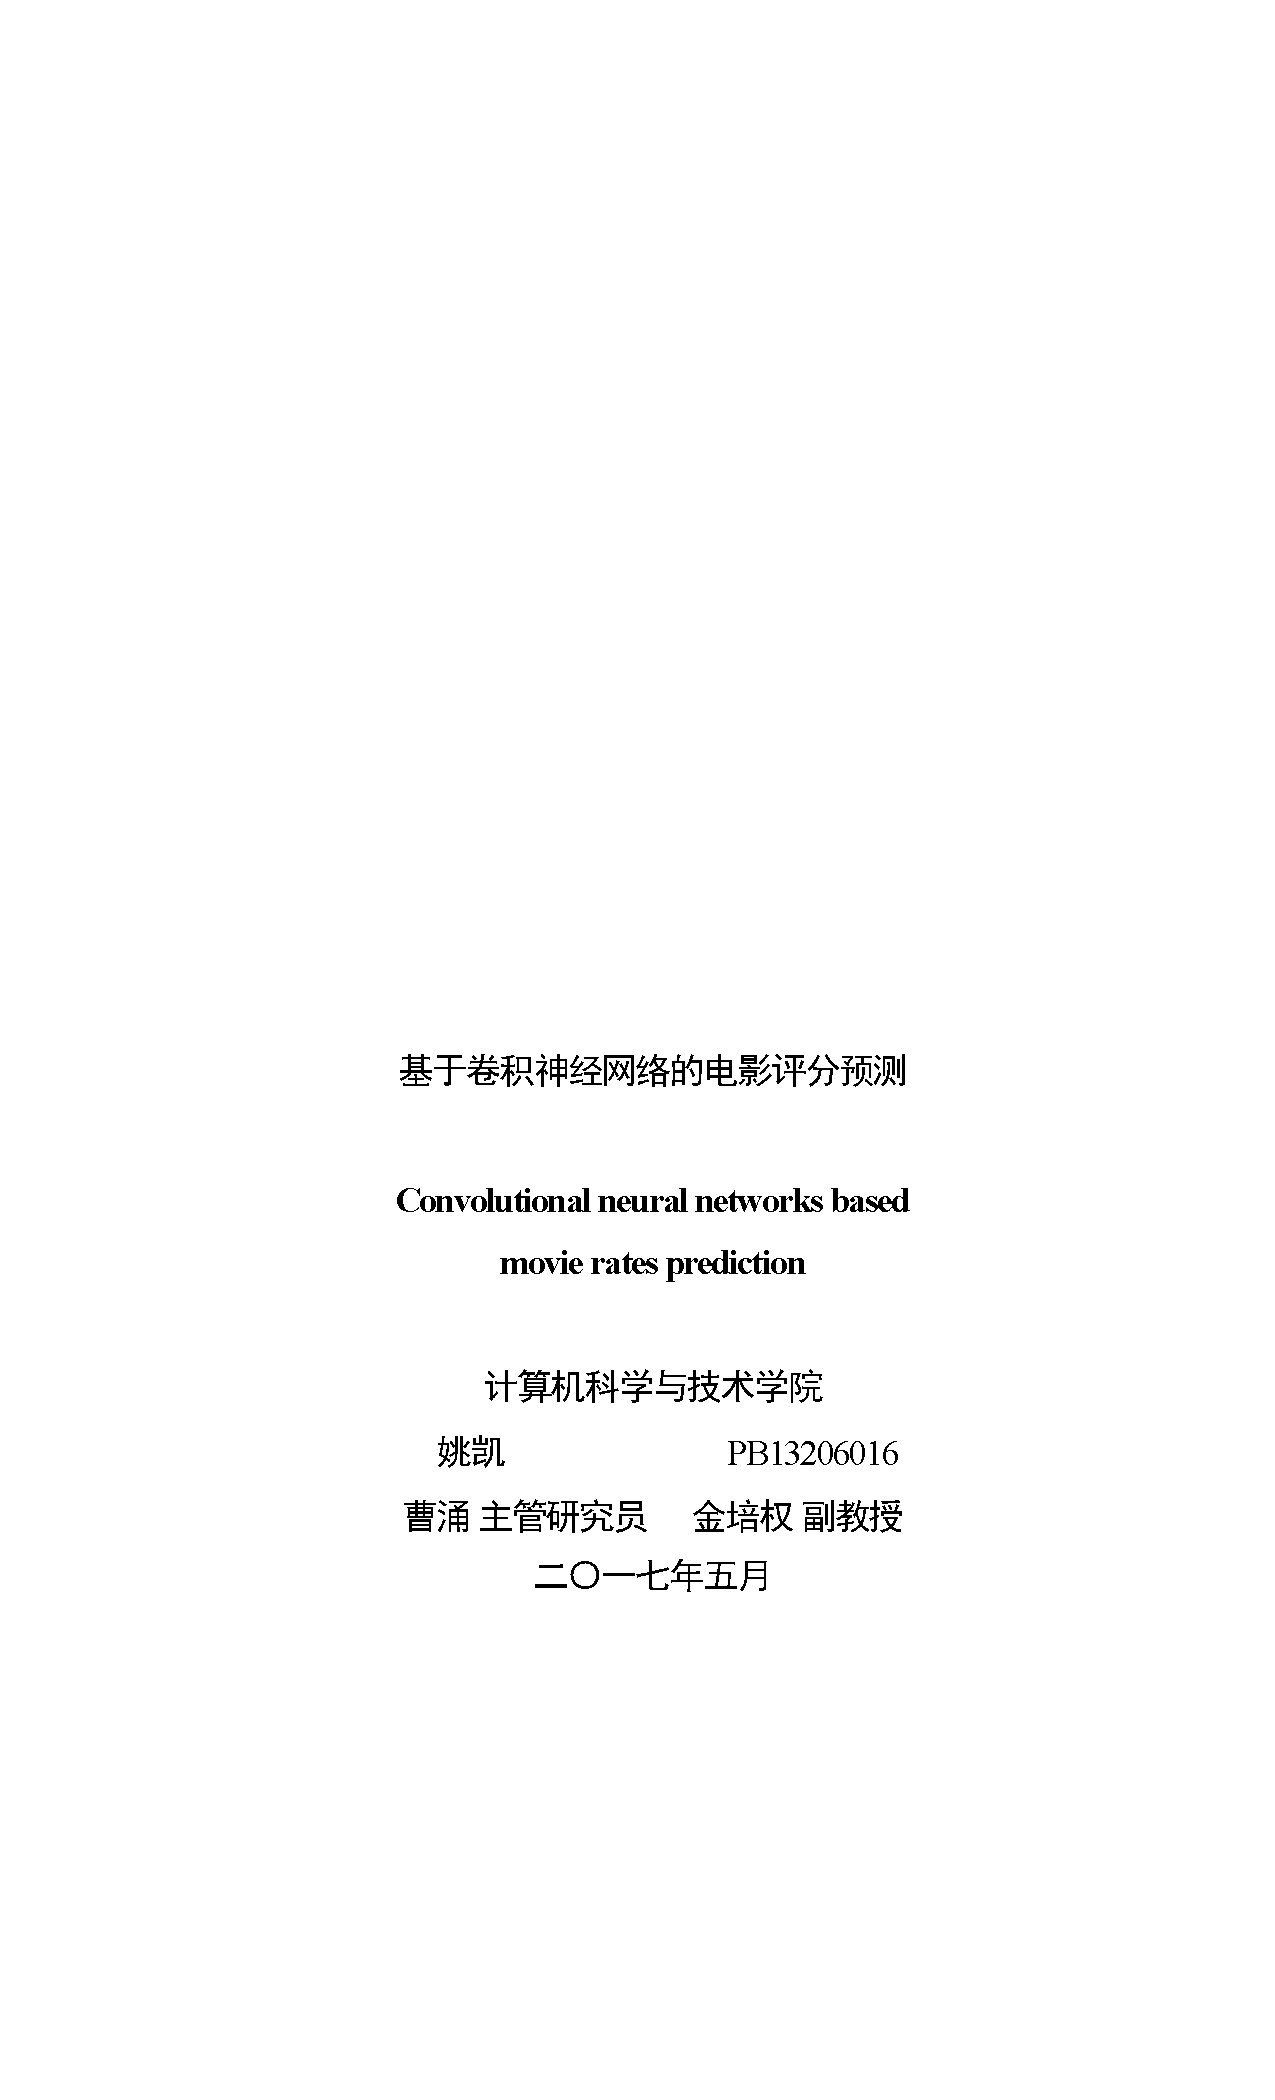
\includepdf[pages=-]{cover.pdf}
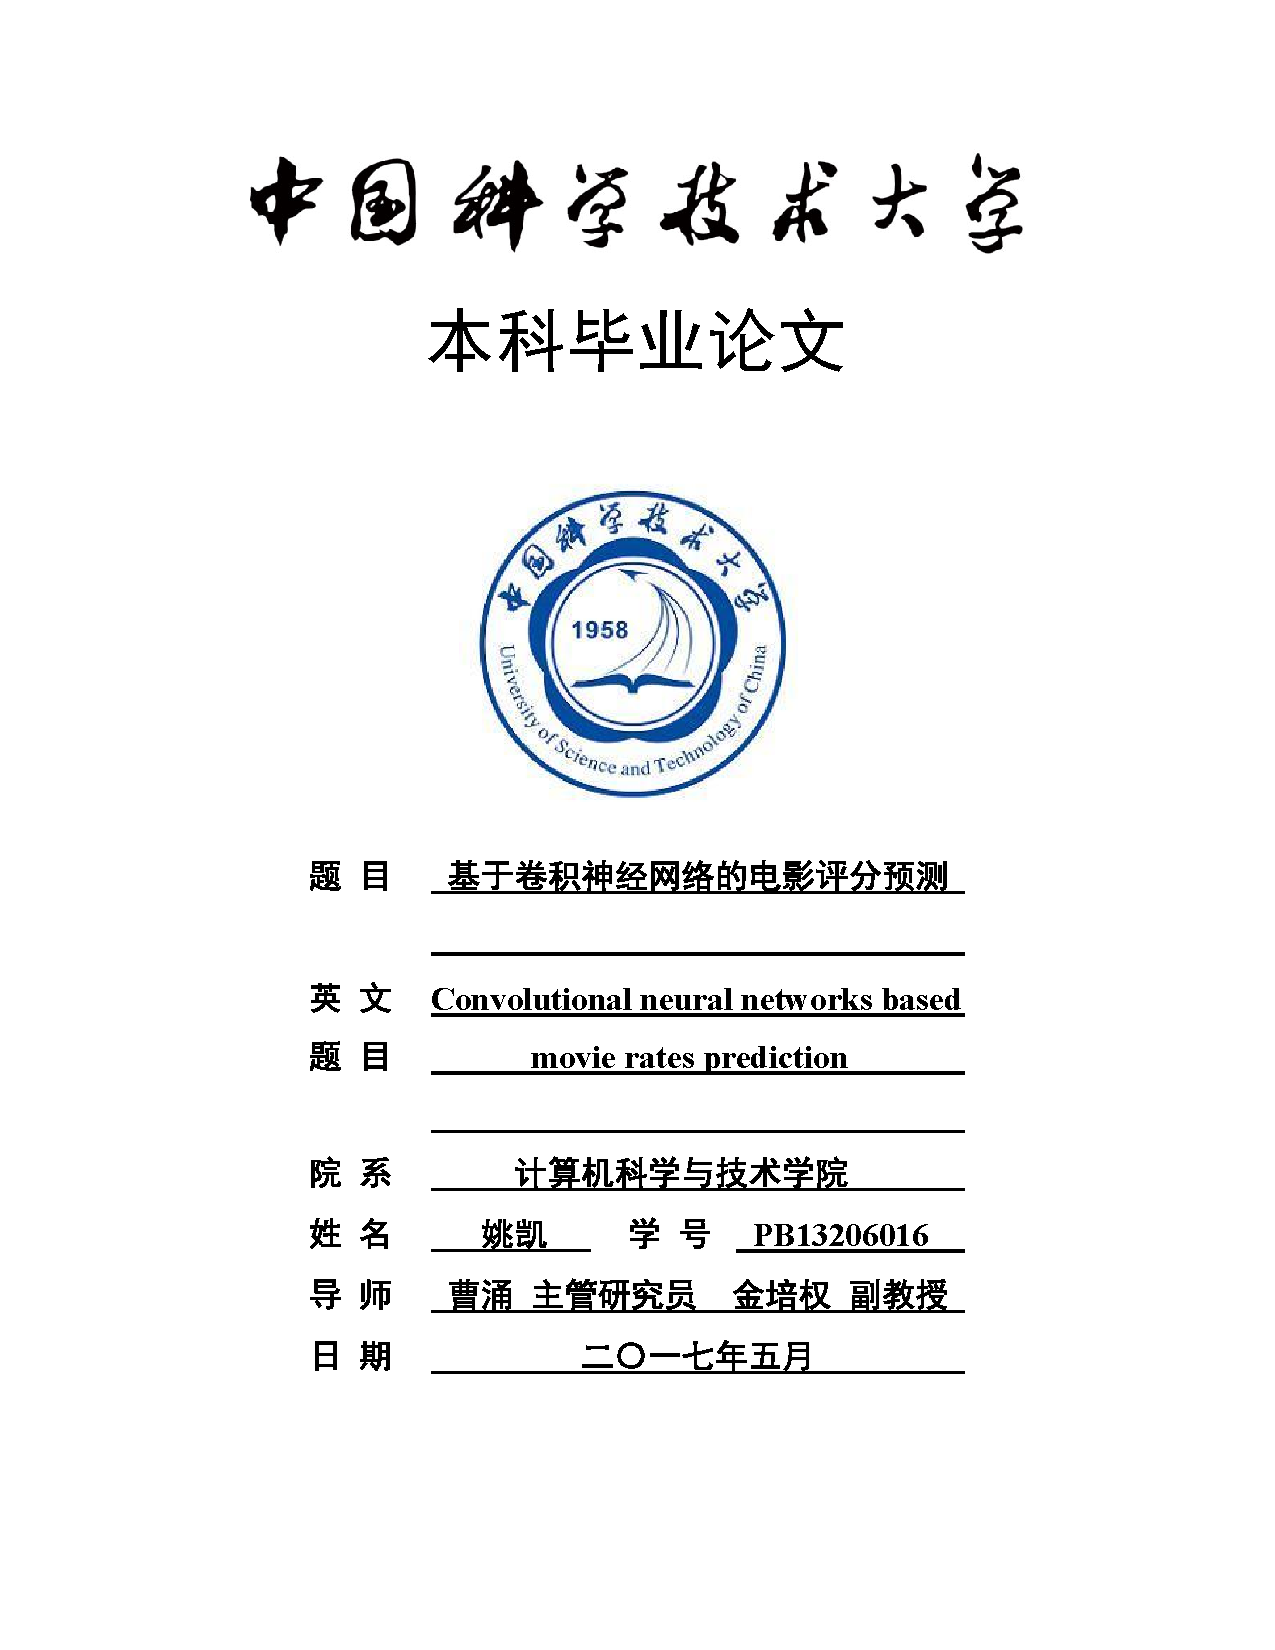
\includepdf[pages=-]{feiye.pdf}
%
% 本科论文:
%   frontmatter: 致谢、目录、中文摘要、英文摘要
%   mainmatter: 正文章节、参考文献
%   appendix: 附录
%
% 硕博论文:
%   frontmatter: 中文摘要、英文摘要、目录、符号说明
%   mainmatter: 正文、参考文献
%   appendix: 附录
%   backmatter: 致谢、发表论文
%

\frontmatter
\begin{acknowledgements}

这里写一堆致谢

\end{acknowledgements}


\tableofcontents
%\listoffigures
%\listoftables
%\listofalgorithms  % 算法索引,如不需要,可直接注释掉本行
% \begin{notation}

\centering
\begin{tabular}{rl}
$\ln x$ & natural logarithm $\log_ex$ \\
$\log x$ & common logarithm $\log_{10}x$ \\
$x\ \mathrm{mod}\ y$ & remainder \\
\end{tabular}

\end{notation}

\begin{abstract}
近年来,随着各种论坛、评论网站不断涌现,越来越多的用户文本出现在网络上。这些文本中很多具有情感倾向,如影评、商品评论、博客评论等。分析这种倾向,有利于获得大众对于电影或商品的评价、了解舆情。因此,对文本进行情感分析的研究有着很强的实际意义。

目前对文本进行情感分析的方法有很多,传统的方法有基于词库的方法,使用已知的情感词典;也有基于机器学习的方法,如朴素贝叶斯和支撑向量机。近年来,深度学习的方法也被用在文本情感分析的问题上。卷积神经网络(Convolutional Neural Network,简称为CNN)是一种发源于计算机视觉领域的深度学习算法,因其模型非常适合图像数据的特征而在计算机视觉领域取得了巨大成功。通过使用“词嵌入”(word embedding)的方法,卷积神经网络也被应用于文本领域,在文本分类等问题上取得了成功。

本文以来自豆瓣的中文短评为语料,使用卷积神经网络对其进行情感分析,判断其情感倾向,并由此预测每一条短评对应的评分(星数)。本文采用Word2vec的算法,从分词后的12万句短评和10万篇长评的语料训练出一个中文词语的word embedding。基于训练出的word embedding 将每个词语转化为词向量,在此基础上使用Tensoflow搭建神经网络的模型,进行情感分析。本文重点实现了卷积神经网络的多种结构,同时实现了复发神经网络(Recurrent Neural Network,简称RNN),以及传统算法如朴素贝叶斯和支撑向量机在这一问题上的应用。分析和比较了不同算法的实验结果以及性能。

\keywords{情感分析,深度学习,卷积神经网络}

\end{abstract}

\begin{enabstract}
Many kinds of forums and comment sites appear on the internet in recent years, therefore, more and more user-generated text contents can be found on the internet. A big part of the text contents generated by user have sentiments, for example, movie reviews, product reviews, blog comments, etc. Analysis of the sentiments in user-generated text contents is helpful for getting feedback of certain movie or product from customers. It is also helpful for analysis of people's opinions or attitudes to certain event. Therefore, research concerning text sentiment analysis has practical meaning.

Currently, there is several methods to do sentiment analysis. For example, traditional lexicon based methods, using a sentiment dictionary; machine learning based methods, such as Naive Bayes classifier and Support Vector Machine (SVM). In recent years, deep learning methods are also used in the task of text sentiment analysis. Convolutional Neural Network (CNN) is deep learning algorithm which was originally used in computer vision field, it has gained significant success in computer vision since it is suitable for the data structure of picture. By using the technique of word embedding, we can also use CNN in the field of text. It has already succeeded in sentence classification.

This paper uses a corpus made up of Chinese movie short comments from Douban. We apply CNN models over this corpus to do text sentiment analysis, and predict the rates of each comments correspondingly. We use Word2vec algorithm to train our corpus of over 160 thousand short movie comments and 100 thousand movie review, and get a word embedding dictionary of Chinese words. We build CNN models over the embedded data using Tensorflow to do sentiment analysis and get the rate predictions. We focus on the implementation of different structure of CNN, we also implement a Recurrent Neural Network (RNN) model, and traditional methods such as Naive Bayes and SVM for comparison purposes. This paper compares different performance of each algorithms, and analyses the results.

\enkeywords{Sentiment Analysis, Deep Learning, Convolutional Neural Network}
\end{enabstract}


\mainmatter
\chapter{绪论}

\section{课题背景与意义}
近年来,随着各种社交媒体和论坛的发展,互联网上的影评已经成为了观影者表达观点、进行交流的重要方式。互联网上出现了许多以影评为主要内容的网站、社区,如IMDB,Rotten Tomatoes,以及中文的豆瓣等。在这些网站上每天都产生出大量的来自用户的文本。这些文本中往往包含了丰富的用户情感信息,如用户对某个电影、演员的评价等。这些用户生成的文本是网站了解用户观点,电影制作者进行市场调研的重要资源。

豆瓣、IMDB上的影评都带有对应的评分(打星数),这样的“影评—评分”对可以看做有标注的数据,它们不需要进一步的人工标注,就可以被用作情感分析的语料。另一些博客或论坛性质的网站,则没有要求用户在给出评论的同时打分。图1.1为一些来自互联网的影评示例。
\begin{figure}[ht]
\centering
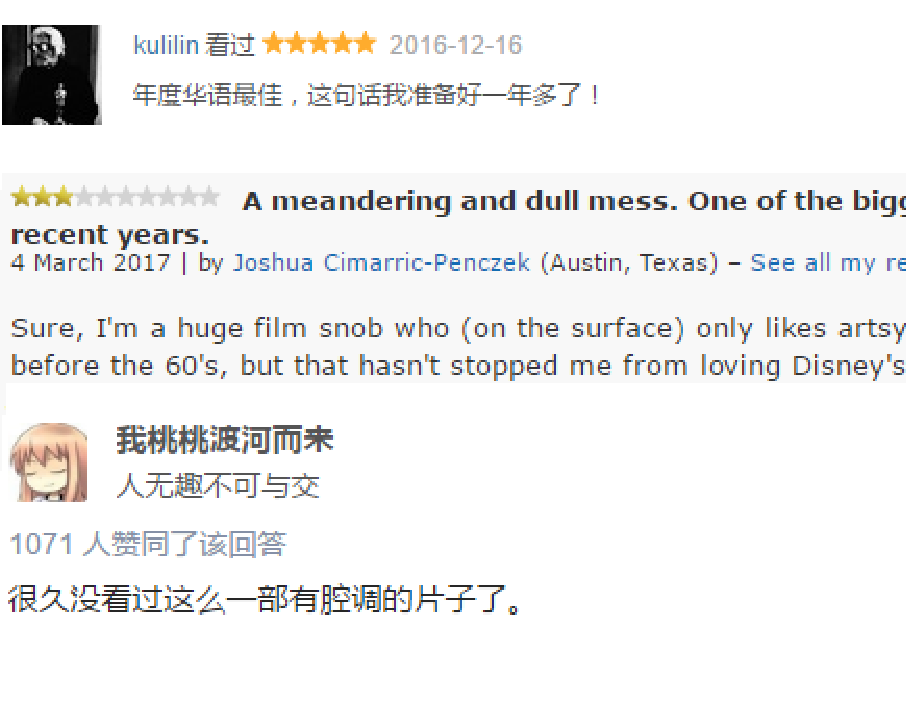
\includegraphics[width=12cm]{Reviews}
\caption{上、中:带有对应评分的影评,分别来自豆瓣和IMDB;下:没有评分的影评,来自知乎} \label{fig:Reviews}
\end{figure}

对影评进行情感分析,将文本形式的影评转化为对应的评分预测,对于网站了解用户对于电影的评价、获得用户反馈和针对用户进行推荐都有着重要意义。在网站不要求用户在评论的同时给出评分的情景下,文本是获得用户情感信息的唯一途径。分析用户文本远不如分析量化的评分容易,如果要人工进行统计分析,工作量会非常大。因此,使用算法对影评进行情感分析,从用户文本中预测该用户对电影的评分,可以大大帮助网站分析来自于用户的数据,收集用户对某一部电影的量化评价。量化后的影评数据方便进行统计,也可以帮助电影制作者进行市场调查。此外,一个用户对各个电影的评分的预测可以很好 地体现该用户的特征,评分预测的结果可以用作推荐系统的输入数据,使网站针对每个用户投放的推荐更为准确。

对于既有影评,又要去用户同时对电影打分的网站,对影评进行情感分析仍然有很重要的意义。因为每个用户对于分数的理解有很大差别,有些用户认为三星是“不错”、“满意”的评分,而另一些则认为是“不满意”、“相当差”。故单纯基于用户打分来收集的对电影的评价往往是有一些偏差的。对文本影评进行情感分析的结果可以在原有评分的基础上起到一个平滑(smooth)的作用,使统计数据更加准确。



\section{相关研究现状}
文本情感分析一直是自然语言处理方向研究的热点,现代进行文本情感分析的方法一般有基于词库(或基于知识)的方法、基于机器学习的有监督学习和无监督学习的方法、以及基于深度学习的方法。

基于词库的文本情感分析方法会采用已知的情感词典(一般由人工筛选出常见的带有情感色彩的单词并进行标注),对于每一个句子,根据其包含的情感单词以及句子的语法结构计算该句的情感倾向\cite{taboada.2011.lexicon}。

现有的机器学习的方法被广泛应用于文本情感分析的问题。监督学习的方法如朴素贝叶斯、最大熵和支撑向量机等,都可以用于情感分析。Pang 等人使用这些方法在来自IMDB的英文影评数据上进行了二分类的实验,其结果证明使用单个单词(unigram)作为特征进行分类就可以取得很好效果,支撑向量机在3折交叉验证中取得了82.9\%的准确率\cite{Pang.2002.ml}。

非监督学习的方法也被应用于情感分析,Peter D. Turney等人使用一种基于情感极性(Sentiment Orientation)的非监督的方法。一个句子的分类由它包含的所有短语的情感方向的平均值决定\cite{turney.2002.thumbs}。每个短语的情感方向由它与单词excellent和poor的相互信息(mutual information)决定。该方法在来自Epinions的410条评论上进行了验证,取得了74\%的准确率。此外,之前所述的基于情感词典的方法也属于无监督学习。

深度学习的模型也被越来越多地应用于情感分析。卷积神经网络(Convolutional Neural Network, 简称CNN)是一种最早发源于计算机图形学的深度学习模型。Yoon Kim等人使用将单词embedding为词向量,再用word vector组成的矩阵来模拟图形矩阵的方法,将CNN 应用在了文本分类的问题上\cite{kim.2014.convolutional}。Yoon等人使用一个简单的只有一层卷积层的CNN在6个数据集上进行了实验,均取得了很好的效果。

\section{本课题主要内容}
本课题使用来自豆瓣的中文短评(每条长度不超过140字,带有评分,可以看作有标注的数据)作为语料,使用卷积神经网络等方法进行文本情感分析,由影评预测对应的评分。

\begin{figure}[ht]
\centering
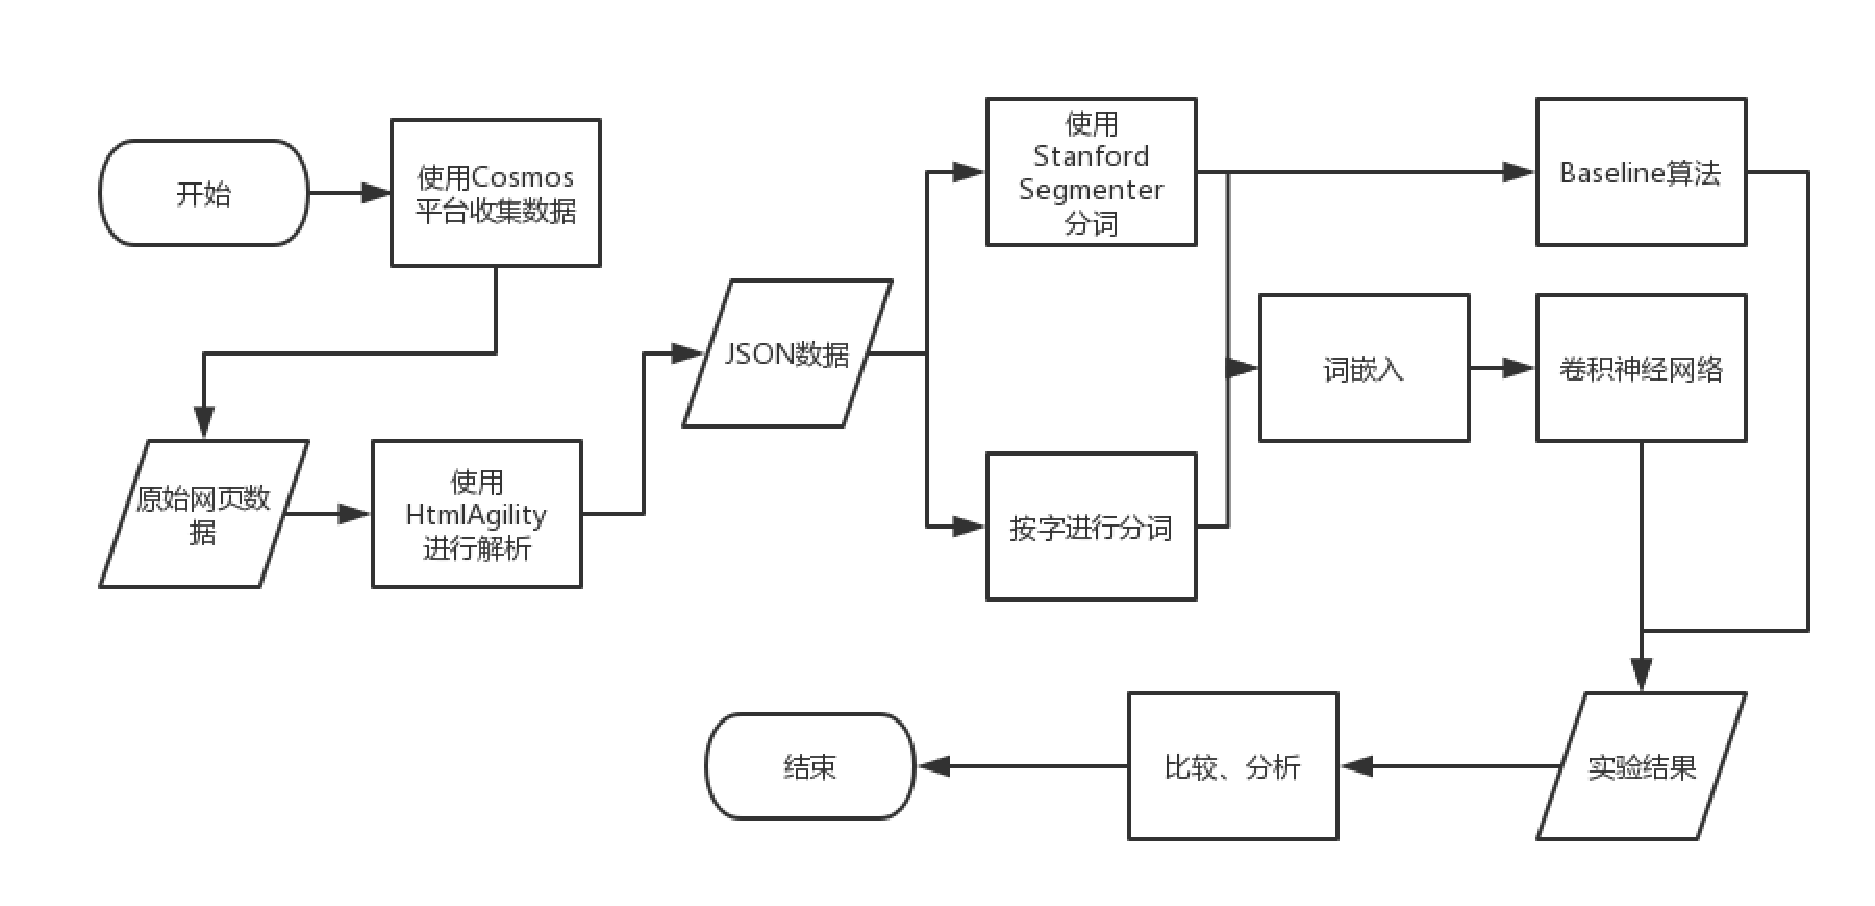
\includegraphics[width=15cm]{Flowchart}
\caption{本课题实验流程图} \label{fig:Flowchart}
\end{figure}


1.	收集数据。使用微软必应搜索的Cosmos分布式处理平台获取了来自豆瓣的16万短评数据以及10万长评数据。

2.	数据预处理。进行中文分词,使用Word2vec算法训练出中文单词的word embedding

3.	建立深度学习模型,调整网络结构,找到适合中文影评数据的模型;实现朴素贝叶斯等传统算法,作为比较。

4.	比较和分析实验结果

本文的组织如下:第一章为绪论,介绍选题的背景和意义,简述当前相关领域研究状况和本课题主要工作;第二章介绍了文本情感分析的相关定义,以及基于词库的方法和基于机器学习的方法;第三章介绍了深度学习的方法在文本情感分析问题上的应用,详细介绍了用于文本分类的卷积神经网络,包括其模型细节和具体算法;第四章介绍了使用卷积神经网络进行影评分类实验的数据集和实验设置;第五章列出了实验结果,并对baseline实验以及多组卷积神经网络的实验结果进行了对比和分析。

\chapter{文本情感分析}
文本情感分析(Sentiment Analysis),也被称为意见挖掘(Opinion Mining),是指对对文本中的主观信息进行辨认、提取和量化。文本情感分析被广泛地应用在用户评论、调查的反馈、网络和社交媒体内容上。一般情况下,文本情感分析的目标是判断文本的作者的(对于某一个主题的)情感倾向。进行情感分析的方法有很多,常见的方法有基于词库的方法,基于机器学习的方法如朴素贝叶斯和支撑向量机等等。

\section{基于词库的方法}
基于词库的文本情感分析方法(Lexicon based method)使用已知的情感字典,这样的情感字典包含情感词以及对应的情感极性。在已有先验的情感词与对应的极性时,可以计算这些情感词在测试句子中出现的次数。一个测试句情感倾向为正向的概率可以计算为 $P(+|D)=\frac{a}{a+b}$, 其中 a和b分别是正向词语和负向词语在该测试句子中出现的次数。

基于词库的方法的优点在于不需要已经标注的数据,因此适用的场景比较广。它的缺点在于,必须存在合适的情感字典,且方法的准确率很依赖于情感字典的质量。对于纯粹以情感词的数目来判断句子情感倾向的方法,没有办法处理句子的复杂语义结构,如“不是很好”这样的情况。

\section{基于机器学习的方法}
\subsection{朴素贝叶斯分类器}
朴素贝叶斯分类器(Naïve Bayes Classifier)是一种条件概率模型,给定一个测试句子,通过计算这个句子属于每一个类别的条件概率来对句子进行分类。贝叶斯分类器中句子的表示是“一袋子词”(Bag of word), 即将句子看作一个无序的词的集合。只考虑每个词的出现次数,不考虑词的相对位置。贝叶斯分类器假设给定一个类别的条件下,每个单词的出现概率都是相互独立的,即$P(w_i|C)$相互独立。在这个假设下,句子属于某一个类别的条件概率就可以通过计算它的每个单词属于该类别的联合概率分布得到,如下:
\begin{equation} \label{eq2.1}
P(C_j|D)=\frac{P(w_1,...,w_n|C_j)*P(C_j)}{P(w_1,...,w_n)}\\
        =\frac{P(C_j)*\prod_{i=1}^{n}P(w_i|C_j)}{\prod_{i=1}^{n}P(w_i)}
\end{equation}
朴素贝叶斯分类器用于情感分析的算法如下:

\begin{algorithm}

\emph{Training Process}\;
\For{$j\leftarrow 1$ \KwTo $class\_num$}{
    \For{$i\leftarrow 1$ \KwTo $vocab\_size$}{
        $count(w_{i}, C_{j})\leftarrow$number of word $w_{i}$ in sentences of class $C_{j}$\;
    }
    $count(C_{j})\leftarrow$number of sentences of class $C_{j}$\;
    $word\_count(C_{j})\leftarrow$number of word in sentences of class $C_{j}$\;
    $P(C_{j})\leftarrow\frac{count(C_{j})}{\sum_{j=1}^{class\_num}count(C_{j})}$\;
}
\BlankLine
\emph{Predicting Function}\;
\textbf{Input:} a segmented sentence\;
\textbf{Output:} predicted class\;
\For{$j\leftarrow 1$ \KwTo $class\_num$}{
    $score(j)\leftarrow$ $\lg{P(C_{j})}$\;
    \For{$i\leftarrow 1$ \KwTo $sent\_length$}{\label{forins}
        $score(j)\leftarrow$ $score(j)+\lg{\frac{count(w_{i}, C_{j})+1}{word\_count(C_{j})+vocab\_size}}$\;
    }
}
Return $augmax_{j}(score(j))$
\caption{朴素贝叶斯分类器}\label{Naive Bayes}
\label{alog:algorithm2}
\end{algorithm}\DecMargin{1em}

朴素贝叶斯分类器用于情感分析的优点在于只需要比较少的训练数据就可以训练出合理的$P(w_i|C)$。缺点在于它依赖的独立性假设是一个很强的假设,很多时候并不符合数据的实际状况。此外,朴素贝叶斯分类器只考虑每个词语出现的次数,而放弃了每个词语的位置的信息。
\subsection{支撑向量机}
支撑向量机(Support Vector Machine,简称SVM)是一种常用的有监督学习的算法。由于它的每个测试样例的输入必须是一个向量,因此,在使用支撑向量机进行情感分类之前,必须对文本进行特征抽取,将句子转化为向量。Ti.idf是一种常见的特征抽取方法。
\subsubsection{Tf.idf 向量化}
Tf.idf全称为Term frequency-inverse document frequency。与朴素贝叶斯相同,tf.idf也是将文本看作“一袋子词”,只考虑每个词语出现的次数。使用tf.idf进行向量化首先需要对训练数据建立词典,对每个词出现的次数进行统计,选取出现次数多于一个阈值的$m$个词,根据这$m$个词在某一个句子和全部句子的出现次数,来将句子转化为一个$m$维的向量。
Tf指词频,其值通过单词在句子中出现的次数除以句子的长度获得,因为一个词语在句子中出现的次数越多,很有可能代表它占了很大比重;Idf可以通过含有该词语的文档占总文档的比率取倒数再取对数得到,因为一个词语如果出现的次数非常多,如汉语中的“的”,则它实际上含有的信息很少,不能作为句子的特征。而出现次数较少的词则含有更多的信息,如果一个词只在很少的几个句子中出现,这几个句子很有可能具有很高的相似度。Tf.idf向量化的结果的每一位由对应单词的tf和idf相乘得到。
\subsubsection{使用支撑向量机进行情感分析}
支撑向量机的目的是找到一个超平面(hyperplane,从而将训练数据最优地分割为两类。为了使这个超平面是最优的,对于每一个类别,支撑向量机算法寻求让最多的该类别的数据点处于超平面的一侧,且最大化超平面的宽度(margin,超平面每一边距离它最近的点到该超平面的距离)。

对于一个二分类的问题,如果训练数据是线性可分的,那么可以找到两个相互平行的超平面将这两类数据完全分隔开,且这两个超平面之间的距离最大化。这样,两个超平面之间的距离就是margin,而要求的最优的超平面就位于这两个平行的超平面的正中间。将输入数据表示为$(\textbf{x}_i, y_i)$, $i=1,..., n$, $y \in \{-1,+1\}$。在进行正规化之后,两个平行的超平面可以表示为$\textbf{w}*\textbf{x}+b=-1$ 和$\textbf{w}*\textbf{x}+b=+1$。 要使两个超平面之间的距离最大,就需要最小化$||\textbf{w}||$,故问题转化为:
\begin{equation} \label{eq2.2}
“Minimize\ ||\textbf{w}||\ subject\ to\ y_i(\textbf{w}*\textbf{x}_i-b)\ge 1,\ for\ i=1,...,n”
\end{equation}

在处理实际问题时,训练数据常常是不线性可分的。通过引入Soft Margin,允许一部分点在两个超平面之间,可以使支撑向量机能够处理这样的问题。Soft Margin的支撑向量机要求在最大化margin宽度的同时,最小化处于两个超平面之间的点到对应超平面的距离(即最小化这些点的误差)。问题转化为最小化函数:
\begin{equation} \label{eq2.3}
J(\textbf{w},b)=[\frac{1}{n}\sum_{i=1}^{n}max(0,1-y_i(\textbf{w}*\textbf{x}_i-b))]+\lambda ||\textbf{w}||^2
\end{equation}

由此得到线性二分类支撑向量机的算法:
\begin{algorithm}

\emph{Training Process}\;
Use tf.idf to transform all text data to vectors.\;
Random initialize $w$ and $b$\;
$\eta_t\leftarrow$ learning rate at time $t$\;
\For{$i\leftarrow 1$ \KwTo $epoch\_num$}{
    $\textbf{w}_{t+1}\leftarrow$$\textbf{w}_t-\eta_t\bigtriangledown_{\textbf{w}_t}J(\textbf{w},b)$\;
    $b_{t+1}\leftarrow$$b_t-\eta_t\bigtriangledown_{b_t}J(\textbf{w},b)$\;
}

\BlankLine
\emph{Predicting Function}\;
\textbf{Input:} a segmented sentence\;
\textbf{Output:} predicted class\;
Use tf.idf to transform input sentence to a vector $x_{i}$\;
Return $sgn(w * x_i + b)$
\caption{支撑向量机}\label{SVM}
\label{alog:algorithm1}
\end{algorithm}\DecMargin{1em}


支撑向量机通过一个核函数(kernel function)将输入数据映射到一个高维的特征空间,通过使用非线性的核函数,如RBF函数,可以得到非线性的分类器。上述的支撑向量机算法只适用于二分类的问题,对于多分类问题,可以使用one-against-one的方法,对每两个类别组合都建立一个二分类的支撑向量机分类器,一共建立$\frac{class\_num * (class\_num - 1)}{2}$个SVM分类器;或者使用one-against-all,对每个类别,建立一个该类别与其他所有类别之间的分类器。

\section{小结}
本章对文本情感分析的定义进行了说明,并且对目前常见的几种文本情感分析的方法进行了介绍。首先对于传统方法中常用的基于情感字典的方法,本章进行了简介和优缺点分析;对于目前非常流行,本课题也会采用做baseline实验的机器学习方法朴素贝叶斯分类器和支撑向量机,本章较详细地介绍了其原理和算法。

\chapter{基于深度学习的文本情感分析}
\section{关于神经网络}
神经网络是一种模仿人类大脑运行模式设计的算法。神经网络由多个层(layer)组成,每层有多个神经元。运算在每个神经元中进行,通过数据在神经网络中流过模仿神经信号的传递。神经元中的运算一般会包括线性运算和一个非线性的激活函数,也有特殊的pooling层和dropout层。以一个全链接层(Full-connected layer的)为例,隐藏层中的每一个神经元接受上一层的所有输出作为它的输入$\textbf{x}$,在进行了线性运算$\textbf{w}* \textbf{x}+b$之后,经过一个非线性激活函数$f$,得到输出$f(\textbf{w} * \textbf{x} + b)$作为输入传到下一层。
\begin{figure}[ht]
\centering
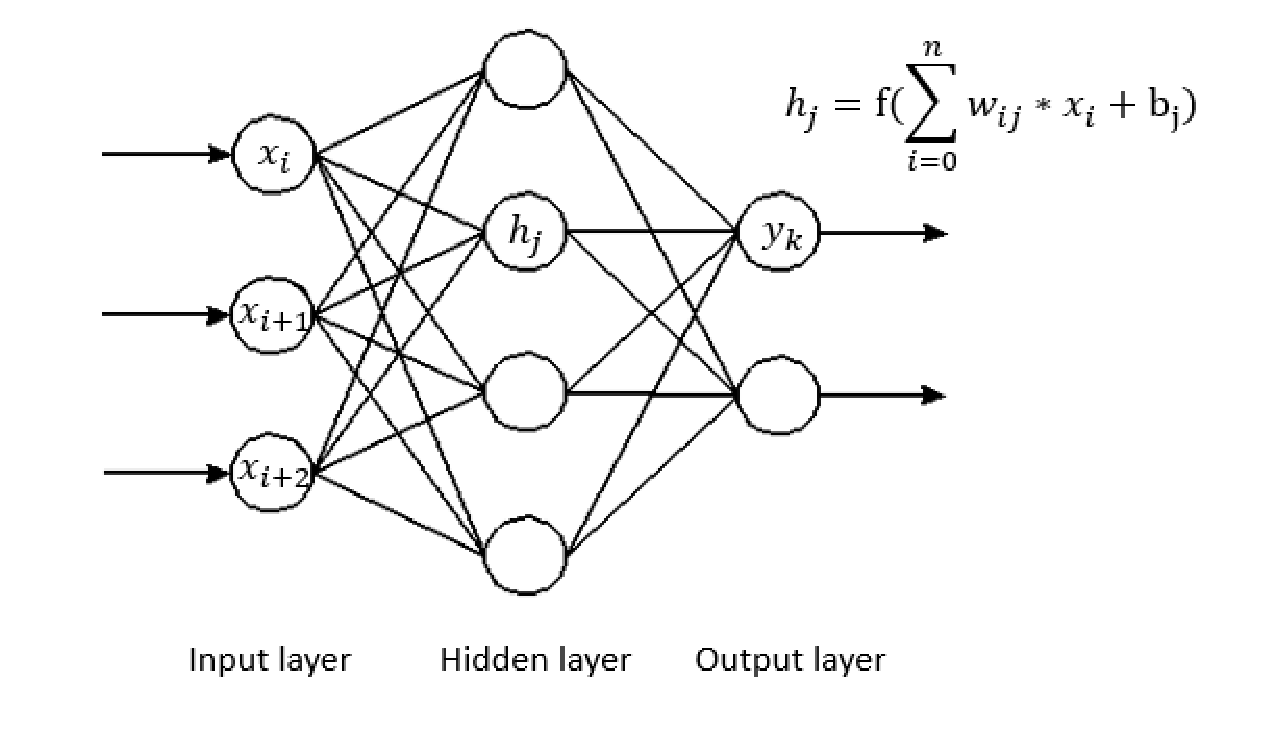
\includegraphics[width=15cm]{FullConnected}
\caption{一个单全链接隐藏层的神经网络} \label{fig:FullConnected}
\end{figure}

神经网络具有非常强的表达能力,具有一个隐藏层的神经网络,在有足够多的神经元数目时可以模仿任意的函数(函数的值域必须在一个有限的区间内)。故近年来神经网络被广泛应用于模式识别、分类等领域,得到了广泛的研究,涌现了如卷积神经网络、复发神经网络等网络结构。通过词嵌入的方法,可以将单词表示为一个固定维数的向量,从而让文本数据可以作为神经网络的合适输入,这样神经网络也可以用于像文本分类这样的问题中。


\section{词嵌入}
对于图像、声音相关的任务,一般都是处理稠密的、高维的输入数据,例如图像数据的像素级别的数据。但涉及到自然语言处理的问题时,传统的方法只能将每个单词表达为一个离散的原子的符号,如“猫”这个词表示为Id234,“狗”这个词表示为Id245。这样的表达只包含很少的信息,且忽视了不同单词间可能存在的关系,如 “猫”和“狗”会被认为是没有关系的两个符号。这样的表达方法还会导致数据非常稀疏,进一步导致需要很多的数据量才能成功训练出统计模型。

词嵌入(word embedding)可以很好地解决上述的问题。词嵌入指将单个词语映射到高维特征空间(一般100到300维)的一个向量。单词之间的相互关系在词向量中可以得到体现,两个单词的相似度一般可以通过计算其词向量的cosine相似度得出。进行词嵌入的算法有两种:基于计数的方法在一个大的语料里统计出一些单词和它的邻居互相同时出现的次数然后将统计结果映射到一个小的、稠密的向量中;预测模型则是建立一个直接从一个词的邻居中预测出这个词的模型,在这个模型的过程中训练出一个最优的词向量。

Word2vec是一种常用的高效率的词嵌入的算法,它是基于预测模型的算法,有Skip Gram和Continuous Bag of Word两种算法供选择,其区别在于预测模型的结构不同。本课题的词嵌入是使用Word2Vec训练出来的。

\section{卷积神经网络}
\subsection{卷积神经网络的结构}
卷积神经网络(Convolutional Neural Network,简称CNN)是一种特殊的神经网络结构,最初被应用在计算机视觉的领域。因为其模型结构非常适合图像数据的特征,卷积神经网络在计算机视觉领域取得了巨大成功,近年来,也被应用于自然语言处理领域的语义理解、语言模型、文本分类等问题上。

与全链接的神经网络层不同,卷积层的每个神经元并不以上一层的全部输出作为输入,而是只取局部的输出。卷积神经网络使用卷积核(convolutional kernels,又称为过滤器filters),每个卷积核只对应很小的感知域(receptive fields,大小可以为2 * 2, 3 * 3等),但这个感知域会贯穿输入数据的深度(输入的第三维,对应图像数据的channel)。对于图像数据而言,第一层卷积隐藏层的每一个神经元,只对应对应图像输入的一个小的像素块,其大小等于卷积核的尺寸,包含全部的RGB三通道。这样的一个神经元只包含其感知域的输入数据的权重参数,只处理输入数据中的一小块局部数据并产生它的输出。

卷积层的另一个特点是参数共享。对于同一个卷积核的全部神经元,其参数是相同的,故卷积神经网络可以理解为一个卷积核在输入数据上进行“滑动”,不断进行卷积运算并产生一个二维的输出。由于每个卷积层一般会有多个卷积核(同一大小的卷积核可以有多个,随机初始化它们的参数以训练出不同的卷积核),所以每个卷积层都会接受一个三维的输入,并给出一个三维的输出(多个卷积核的输出结果叠加形成第三维)。这样,一个卷积层的输出在经过线性整流层(Rectified Linear Units layer, ReLU layer)作非线性化处理后,可以很方便地作为输入进入下一个卷积层。

卷积神经网络层相较于全链接层的一个优势在于不会有“纬度诅咒”的问题。例如,对于一个100*100*3的输入数据(图像数据或者经过词嵌入的文本数据都有这样的结构),在第一个隐藏全链接层中的每一个神经元都需要有 100 * 100 * 3 = 30000个权重参数,如果该层有100个神经元,则会产生100 * 30000 = 3000000个权重参数。而对于一个有128个2 * 2的卷积核的卷积层,只需要2 * 2 * 3 * 128 = 1536个权重参数 。
卷积神经网络的另一个优势在于可以提取输入数据的局部特征,每个卷积核只处理输入数据的一小块,多层卷积层后,图像数据的信息得到更好的归纳。

\subsection{卷积神经网络应用于文本问题}
卷积神经网络在计算机视觉领域的成功与图像数据的结构特点密切相关。与图像数据由像素点组成不同,文本数据由单词组成,因此,卷积神经网络不能直接应用于文本数据上。必须将文本数据映射成一个维度不高、稠密的矩阵数据形式。

通过对文本数据进行词嵌入,我们可以用一个句子中所有单词的词向量拼接出一个二维的矩阵。使用多个不同的词嵌入(要求词向量的维度相同),可以得到多个这样的二维数据,从而堆叠出一个三维的数据(第三维对应图像数据中的channel)。这样,文本数据转化成为卷积神经网络可以接受的输入。

应用于文本数据输入的卷积神经网络与图像数据的卷积神经网络存在着一些差别,主要在于卷积核的大小。应用于图像数据的卷积神经网络卷积核大小可以为2 * 2,3 * 3,2 * 3等,长和宽没有严格的限制。但对于接受文本数据输入的卷积层,其卷积核的宽度一般等于词向量的宽度,即卷积核会占满词向量这一维,只在句子长度这一维上滑动。这是因为每一行都是原输入数据中的一个单词,如果在单词内部使用更小的卷积核进行卷积运算的话,相当于“破开”了一个单词。在不了解词向量每一位的意义的情况下,“破开”词向量并不合理。此外,卷积核的长度(对应每次进行卷积运算时覆盖的单词数)也不会太短,一般很少会超过五。因为文本中每个单词相较于图像中的像素,粒度要大一些,如果卷积核的感知域覆盖了太多单词,就不存在“提取局部特征”的优势了。

应用于文本领域的卷积神经网络与传统的N-gram方法有相似之处,它们都会提取连续出现的单词作为句子或者文档的局部特征。相较于传统的N-gram方法,卷积神经网络有如下几个优势:首先卷积神经网络不用像n-gram那样简历非常大的词典(在比较大的语料上,3-gram已经需要建立庞大的词典才能正常工作);此外,卷积神经网络可以利用GPU的硬件优势,进一步得到加速,因为卷积运算作为一个计算机图形学中非常基础的运算,通常在GPU的硬件层面上就会给予特别支持。

\begin{figure}[ht]
\centering
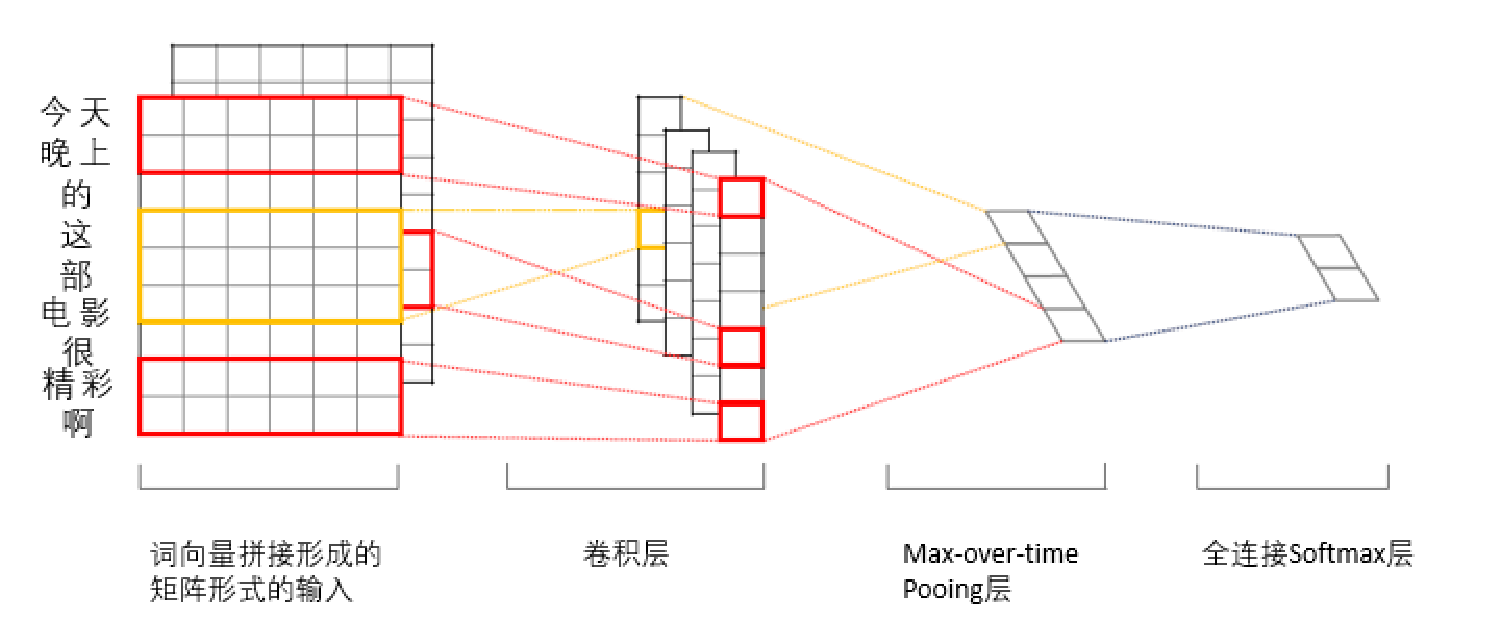
\includegraphics[width=15cm]{CNN}
\caption{卷积神经网络应用于文本分类,图像部分引用自\cite{kim.2014.convolutional}} \label{fig:CNN}
\end{figure}

\subsection{具体算法}
用$w_i\in \mathbf{R}^k$来表示句子中的第i个单词对应的长度为$k$的词向量,一个长度为n的句子可以表示为:
\begin{equation} \label{eq3.1}
x_{1:n} = [x_1; x_2;...; x_n]
\end{equation}
使用$x_{i:i+j}$来表示词向量$x_i, x_{i+1}, …, x_{i+j}$连接的结果。一个卷积核$w\in \mathbf{R}^{h*k}$,将作用在一个包含h个单词的“窗口”上来产生一个特征。例如,一个特征$c_i$可以从单词$w_{i:i+h-1}$中通过下式产生:
\begin{equation} \label{eq3.2}
c_i = f(\textbf{w}*\textbf{x}_{i:i+h-1} + b)
\end{equation}	
这里的b为偏差值(bias),f是一个非线性函数(如ReLU)。随着窗口在整个句子上滑动,这个卷积核可以作用在每一个可能的窗口上,产生了如下的特征序列:
\begin{equation} \label{eq3.3}
\textbf{c} = [c_1, c_2, ..., c_{n-h+1}]
\end{equation}	
$\textbf{c}\in\mathbf{R}^{n-h+1}$。在卷积层得到的特征序列上加以一个max-over-time pooling,只保留特征序列中的最大值$\^{c}=max\{\textbf{c}\}$,这是为了只保留每个特征序列中最重要的特征。在经过max-pooling层后,每个卷积核只保留了一个特征。多数个卷积核(可以有不同的窗口大小)会产生一系列的特征,这些特征连接起来,作为最后的全连接Softmax层的输入。
此外,在输入层和max-pooling层之后,我们的模型中加入两个dropout层。Dropout层会随机地筛选出一部分输入,将其值设为0,再进行输出。Dropout层的目的是通过随机去掉一些神经网络中的信号传递以减少过拟合。

\section{复发神经网络}
复发神经网络(Recurrent Neural Network,简称RNN)是另一个常见的神经网络结构,复发神经网络中的信号不仅会向前传播,而且会传回给自身,因此被称为recurrent。具体到文本问题上,复发神经网络单元每次在处理完一个单词后,除去产生一个输出外,还会记住一部分信息。在处理下一个单词时,会根据当前输入以及之前记住的信息来产生下一个输出,并更新记住的信息。

Long Short Term Memory,简称LSTM,是一种特殊的复发神经网络。它使用一个“遗忘门”来选择性的忘记一部分记住的信息,同时使用一个“输入门”来记住一部分非线性话处理后的上一轮留下的输入。LSTM的优势在于他可以处理长距离的依赖关系。

复发神经网络由于能够在文本数据流过网络时“记住”一些之前的信息,因此,可以很好利用到输入数据的全局特征和顺序特征。在文本分类这个问题上,他可以利用词语的位置特征,挖掘整个句子的信息。复发神经网络在文本相关的问题上一直有很好的表现。

由于本课题只使用LSTM作为一个用于比较的实验,重点仍然是卷积神经网络在情感分析问题上的应用,故只简单地介绍LSTM的原理。关于RNN和LSTM的具体内容,可以参考\cite{socher.2013.recursive}和\cite{sundermeyer2012lstm}。

\section{小结}
本章对深度学习的方法如何应用于情感分析问题进行了说明。首先简介了神经网络的基本原理,然后词嵌入技术进行了说明;之后对就卷积神经网络相关内容进行了详细介绍包括其原理、如何应用于文本问题以及具体的算法;最后简介了作为baseline实验的LSTM的基本原理。

\chapter{基于卷积神经网络的影评分类实验}
\section{数据集与预处理}
\subsection{数据的获取与概况}
本论文采用的数据集是来自豆瓣的中文影评数据。使用微软必应(Bing)搜索的Cosmos分布式处理平台获取。来自Cosmos的数据是原始的HTML 文本,使用HtmlAgility库对其进行解析,提取出有用的影评、评分等信息,整理成JSON格式的文件。数据的基本信息如表格\ref{tab:comment count}所示。

\begin{table}[H]
\centering
\caption{数据数量表格} \label{tab:comment count}
\begin{tabular}{c|c|c|c}
    \hline
    全部短评数量 & 全部长评数量 & 短评来源用户数量 & 短评对应电影数量\\
    \hline
    124591 & 100000 & 42517 & 4887\\
    \hline
\end{tabular}
\end{table}

整理生成的短评数据示例如表格\ref{tab:comment format}所示。
\begin{table}[H]
\centering
\caption{短评数据示例} \label{tab:comment format}
\begin{tabular}{c|c|c|c|c|c|c}
    \hline
    Text & Username & Rate & Cid & Vote & MovieName & MovieId\\
    \hline
    这么高分我有点不懂 & X.Lee & 3 & 1005243594 & 12 & 拿起枪的简 & 10760385\\
    \hline
\end{tabular}
\end{table}

短评数据每条的长度不超过140个字符,每条都带有对应评分(1到5星);长评数据没有字数限制,同样每条都包括1到5星的评分。

选择来自豆瓣的中文影评作为语料的优势在于,短评和长评都可以看作有标注的数据,这就意味着我们不再需要再人工地对数据进行标注就可以在它们上面进行有监督的学习。此外,豆瓣的短评有长度的限制,易于转换为固定大小的输入矩阵,故我们使用短评作为主要的实验数据。对于获取到的长评数据,虽然它们也是有标注的数据,但由于它们之间长度相差很大,而且相对于情感信息比较密集的短评,长评中可能有很多谈论具体电影情节的,不带情感色彩的内容。所以本论文不直接使用长评数据进行实验,而是使用他们进行了词嵌入的训练。因为长评数据本身的数据量很大,其语境和用语习惯与短评非常接近,所以使用它们作为训练词嵌入的语料非常适合。

\subsection{分词与训练词嵌入}
获得了JSON格式的数据后,由于JSON中的Text域是原始的短评文本,所以还需要进行分词和训练词嵌入才能将这些数据转化为神经网络可以接受的形式。本论文采用的中文分词工具是斯坦福大学自然语言处理研究组的Stanford Word Segmenter,该分词工具基于的算法是使用条件随机场(Conditional Random Field)去做sequence model。

将短评数据和长评数据进行分词后,将其作为输入数据进行词嵌入的训练。训练词嵌入采用的算法是基于Continuous Bag of Word的Word2vec,这是一种高效率的词嵌入训练算法。本论文使用gensim库中对Word2vec的实现,选取词向量长度为100,从短评和长评数据中训练出了中文词语的词嵌入。

\subsection{实验设置}
本论文的实验分为两种,第一种是由中文电影短评预测该短评对应的评分(1到5星),本论文以短文本五分类的方法来实现对影评的预测;第二种是将五分类的中的3星评论去除,以1星和二星评论作为负面评论,四星和五星评论作为正面评论,由短评的内容预测其评论的倾向(正面还是负面),将问题转化为个短文本二分类来做。

在使用短评数据进行实验之前,我对短评根据其作者发布的影评数量进行了筛选,只保留了发表影评数量超过5的较活跃用户的影评。符合要求的影评共67255篇。抽取其中60000篇,进行了shuffle后按表格\ref{tab:data divide}划分了训练集,验证集和测试集(由于第二类实验需要去除三星的评论,故第二类实验的数据规模与第一类有所区别)

\begin{table}[H]
\centering
\caption{实验数据划分表格} \label{tab:data divide}
\begin{tabular}{c|c|c|c}
    \hline
     &训练集 & 验证集 & 测试集\\
    \hline
    评分预测实验 & 40000 & 10000 & 10000\\
    \hline
    二分类实验 & 28204 & 7059 & 7016\\
    \hline
\end{tabular}
\end{table}



\section{不同的卷积神经网络结构}
对于实验中的所有神经网络模型,均采用每个尺寸128个卷积核的设置。卷积核宽度固定等于词向量宽度,如卷积核长度为1、2、3,则长度为1、2、3 的卷积核各有128个,共384个不同的卷积核;在输入数据和pooling层后各设置一个dropout层,dropout的比率在0.0,0.3,0.5这三个档位进行网格实验,选出最优的一组。

实验设置在卷积神经网络的输入数据如何断句、通道数以及卷积网络的层数等超参数的设置上有所分化,主要分为以下几类实验:
\subsection{单层单通道}
结构如第三章中所述,只有一层卷积层,卷积的输出经过pooling和dropout直接传给最后进行分类的全连接Softmax只使用一个词嵌入,故卷积神经网络的输入的第三维宽度只有一,对应图像数据只有一个通道。这里的词嵌入层也作为神经网络的一部分,词向量的值也会通过backpropagation更新。

我们使用单层单通道网络在词语层面(使用中文分词器断句)和字层面(在每个字断句)的输入上都进行了实验,其中词语层面的词嵌入使用Word2vec的训练结果初始化,字层面则随机初始化。

\subsection{单层双通道}
同样只有一层卷积层,但有两个词嵌入,故传给卷积层的输入第三维大小为2,即有两个通道。这两个词嵌入都使用Word2vec的训练结果初始化,其差别在于只有其中一个在训练过程中保持更新,另一个则始终不变。单层双通道只在词语层面的输入上进行了实验。

\subsection{双层卷积神经网络}
使用两个卷积层,在字层面的输入上进行实验。旨在第一层完成字组合的特征提取,第二层提取更高层面的特征。

\section{Baseline 实验}
本论文进行了三个baseline实验用作对比和分析。分别为朴素贝叶斯分类器,基于Tf.idf特征抽取的支撑向量机,和LSTM神经网络。由于在本文的第二章文本情感分析已经对baseline方法的基本原理进行了介绍,这里只说明具体的实验设置。

朴素贝叶斯分类器使用基于计数的方法计算$P(w_i|C)$和$P(C)$。对于单词的出现次数设置阈值10,即一个单词只有在训练数据中出现的次数超过十次才能被用在预测中。具体的概率的计算方法和算法流程见算法\ref{Naive Bayes}。

支撑向量机使用Tf.idf来进行特征抽取,将句子转化为一个一维的向量。对于Tf.idf的词典设置阈值50,因为向量化的结果的长度等于词典大小,故需要选取一个比较高的阈值以压缩向量长度,选取50为阈值得到的向量长度约2000。使用RBF的核函数,Soft Margin的支撑向量机设置。对于评分预测的五分类的实验,使用one-agains-all的方法,将支撑向量机由二分类拓展为5分类。具体的算法流程见算法\ref{SVM}。

LSTM神经网络使用Tensorflow实现。输入数据为经过词嵌入的得到的词向量序列,单层的LSTM之后,经过一个平均值池化(mean-pooling),对每个词向量的输出取平均值,得到一个长度为隐藏层宽度的一维向量。该一维向量再通过一个Softmax,得到分类的预测结果。

\section{实验结果与分析}
Baseline实验结果如表格\ref{tab:results base}所示。

\begin{table}[H]
\centering
\caption{Baseline实验结果} \label{tab:results base}
\begin{tabular}{c|c|c|c}
    \hline
      & Naive Bayes & SVM & LSTM \\
    \hline
    评分预测(五分类)实验 & 41.54\% & 38.7\% & 43.62\% \\
    \hline
    二分类实验 & 79.64\% & 78.31\% & 81.77\% \\
    \hline
\end{tabular}
\end{table}
卷积神经网络评分预测(五分类实验)实验结果如表格\ref{tab:results5}所示、二分类预测实验结果如表格\ref{tab:results2} 所示。
\begin{table}[H]
\centering
\caption{评分预测实验准确率结果} \label{tab:results5}
\begin{tabular}{c|c|c|c|c}
    \hline
    Filters Sizes & CNN\_char & CNN & CNN\_2\_channel & CNN\_2\_layer\\
    \hline
    1 & 40.41\% & 43.04\% & - & - \\
    \hline
    1,2 & 42.11\% & 44.12\% & 43.29\% & 40.61\% \\
    \hline
    1,2,3 & 42.49\% & 43.28\% & - & - \\
    \hline
\end{tabular}
\note{实验设置见第四章第二、第三节相关内容,CNN\_char指使用按字断句的输入;双通道和双层只在单层的最优设置上进行了实验。}
\end{table}

\begin{table}[H]
\centering
\caption{二分类实验结果} \label{tab:results2}
\begin{tabular}{c|c|c|c|c}
    \hline
    Filters Sizes & CNN\_char & CNN & CNN\_2\_channel & CNN\_2\_layer\\
    \hline
    1 & 77.89\% & 81.42\% & - & - \\
    \hline
    1,2 & 79.74\% & 82.05\% & 81.33\% & 77.29\% \\
    \hline
    1,2,3 & 80.47\% & 81.50\% & - & - \\
    \hline
\end{tabular}
\note{实验设置见第四章第二、第三节相关内容,CNN\_char指使用按字断句的输入;双通道和双层只在单层的最优设置上进行了实验。}
\end{table}

可以看到使用中文分词器分词的效果要好于按字断句,说明对中文语言文本分词的确可以提取出文本中很多的特征。而基于字断句的话,在训练数据不非常大的情况下(40000句仍然只能算比较少的数据量),或是模型复杂程度不够高的情况下,可能会导致一些信息或特征无法被提取出来,因而导致结果不如分词后的数据。但同时也可以注意到,在卷积核的设置包含了3或4这样比较大的窗口时,基于字断句的输入也会有很好的效果。这说明了说明卷积神经网络的确有提取局部特征(在这里体现为提取出字的组合的特征)的能力。

对于同一卷积神经网络结果,不同的卷积核设置也会明显地影响实验结果。对于输入使用分词器断句的实验,准确率在卷积核长度达到2时达到最大,加上长度为3的卷积核准确率反而下降;对于输入使用按字断句的实验,加上长度为3的卷积核后准确率得到了提高,但再加上长度为4的卷积核后(数据未列在上表上)准确率也下降了。给处理文本问题的卷积神经网络增加更大的卷积核可以看作一种Tradeoff,一方面增加更大的卷积核有可能提取出更多的句子特征,另一方面,这样也会使整个模型更加容易过拟合。实验结果表明,在进行了分词的数据上,连续三个中文词语中可以提取的特征已经很少,由此带来的“更容易过拟合”的缺点对结果的影响甚至超过了提取三个连续词语的特征带来的影响。

单层双通道的模型也取得了很好的实验结果,但其最好的结果没有超过单层单通道的最好实验结果。这与我们开始时的期望略有出入,可能是由于双通道的模型更容易过拟合。双层卷积层模型的结果也超过了baseline算法,但落后于单层卷积层的两种模型。这与图像数据领域的结果有很大差别,可能是因为文本数据每个单词相较于图像数据的像素,包含的信息要多得多。因此,即使在单层卷积层的模型也可以提取出很多的信息,也会有很好的结果。而多层之后,反而由于抽象的层数太高、过拟合的机会增大,可能会导致效果反而不如单层的网络。

另外也可以注意到,五分类问题的结果准确率普遍比较低,不超过45\%。这是由于对影评进行五分类本身是一个比较困难的问题,与本论文数据集相近的SST-1数据集(同样是影评数据,分为五类,分别为非常负面、负面、中立、正面和非常正面),目前最前沿的成果也只能达到48.7\%的准确率。这个问题准确率难以提得很高是因为每个影评者自己的指标不同,同样一句影评,对于一些人来说会选择给四星,另一些人则会给五星、三星。此外,中间三档影评的区分度很低。本论文使用的数据集未经过人工筛选,只根据作者发过的影评数设置了一个阈值。故数据集中可能存在评论与打分不符,或是一些没有意义的垃圾信息。这些评论也会对结果产生影响。

\begin{table}
\centering
\caption{Confusion Matrix} \label{tab:confusion}
\begin{tabular}{c|c|c|c|c|c}
    \hline
     & 1 & 2 & 3 & 4 & 5\\
    \hline
    1 & 0 & 306 & 166 & 86 & 61\\
    \hline
    2 & 229 & 0 & 303 & 79 & 22 \\
    \hline
    3 & 280 & 687 & 0 & 992 & 340 \\
    \hline
    1 & 59 & 127 & 647 & 0 & 587\\
    \hline
    1 & 43 & 53 & 153 & 368 & 0\\
    \hline
\end{tabular}
\note{横坐标为Ground Truth,纵坐标为预测值。}
\end{table}

表格\ref{tab:confusion}是五分类问题最后结果的confusion matrix,即预测错误的分布。可以看到,大多数的错误分布在主对角线附近,即出现在相邻的两个分段。尤其是中间二、三、四三个阶段,出现的错误非常多。这印证了我们上一段的分析。

因为五分类的结果准确率较低,难以应用在实际问题中。我们又增加了二分类的试验,可以看到,二分类实验的准确率很高,达到了82\%以上。同时可以注意到,各种模型在二分类问题上的相对表现与五分类的相当,即五分类问题中表现好的模型,在二分类中仍有很好的表现。没有出现只在某一个问题上表现特别好或特别差的异常现象,实验结果与预期相符。

\section{小结}
本章对论文所做的工作进行了说明。首先说明了数据的来源,对数据的预处理,已经实验的总体设置;然后说明了实现的不同神经网络结构的区别;之后,说明了baseline实验的设置;最后,对实验结果进行了总结和分析。比较了卷积神经网络的不同卷积核选取带来的结果差异;比较和分析了单层单通道和更复杂网络结构的实验结果;具体分析了为什么评分预测的准确率较低。

%\chapter{实验结果与分析}
\section{实验结果}
Baseline实验结果如表格\ref{tab:results base}所示;卷积神经网络评分预测(五分类实验)实验结果如表格\ref{tab:results5}所示、二分类预测实验结果如表格\ref{tab:results2} 所示。

\begin{table}
\centering
\caption{Baseline实验结果} \label{tab:results base}
\begin{tabular}{c|c|c|c}
    \hline
      & Naive Bayes & SVM & LSTM \\
    \hline
    评分预测(五分类)实验 & 41.54\% & 38.7\% & 43.62\% \\
    \hline
    二分类实验 & 79.64\% & 78.31\% & 81.77\% \\
    \hline
\end{tabular}
\end{table}

\begin{table}
\centering
\caption{评分预测实验准确率结果} \label{tab:results5}
\begin{tabular}{c|c|c|c|c}
    \hline
    Filters Sizes & CNN\_char & CNN & CNN\_2\_channel & CNN\_2\_layer\\
    \hline
    1 & 40.41\% & 43.04\% & - & - \\
    \hline
    1,2 & 42.11\% & 44.12\% & 43.29\% & 40.61\% \\
    \hline
    1,2,3 & 42.49\% & 43.28\% & - & - \\
    \hline
\end{tabular}
\note{实验设置见第四章第二、第三节相关内容,CNN\_char指使用按字断句的输入;双通道和双层只在单层的最优设置上进行了实验。}
\end{table}

\begin{table}
\centering
\caption{二分类实验结果} \label{tab:results2}
\begin{tabular}{c|c|c|c|c}
    \hline
    Filters Sizes & CNN\_char & CNN & CNN\_2\_channel & CNN\_2\_layer\\
    \hline
    1 & 77.89\% & 81.42\% & - & - \\
    \hline
    1,2 & 79.74\% & 82.05\% & 81.33\% & 77.29\% \\
    \hline
    1,2,3 & 80.47\% & 81.50\% & - & - \\
    \hline
\end{tabular}
\note{实验设置见第四章第二、第三节相关内容,CNN\_char指使用按字断句的输入;双通道和双层只在单层的最优设置上进行了实验。}
\end{table}

\section{结果分析}
可以看到使用中文分词器分词的效果要好于按字断句,说明对中文语言文本分词的确可以提取出文本中很多的特征。而基于字断句的话,在训练数据不非常大的情况下(40000句仍然只能算比较少的数据量),或是模型复杂程度不够高的情况下,可能会导致一些信息或特征无法被提取出来,因而导致结果不如分词后的数据。但同时也可以注意到,在卷积核的设置包含了3或4这样比较大的窗口时,基于字断句的输入也会有很好的效果。这说明了说明卷积神经网络的确有提取局部特征(在这里体现为提取出字的组合的特征)的能力。

对于同一卷积神经网络结果,不同的卷积核设置也会明显地影响实验结果。对于输入使用分词器断句的实验,准确率在卷积核长度达到2时达到最大,加上长度为3的卷积核准确率反而下降;对于输入使用按字断句的实验,加上长度为3的卷积核后准确率得到了提高,但再加上长度为4的卷积核后(数据未列在上表上)准确率也下降了。给处理文本问题的卷积神经网络增加更大的卷积核可以看作一种Tradeoff,一方面增加更大的卷积核有可能提取出更多的句子特征,另一方面,这样也会使整个模型更加容易过拟合。实验结果表明,在进行了分词的数据上,连续三个中文词语中可以提取的特征已经很少,由此带来的“更容易过拟合”的缺点对结果的影响甚至超过了提取三个连续词语的特征带来的影响。

单层双通道的模型也取得了很好的实验结果,但其最好的结果没有超过单层单通道的最好实验结果。这与我们开始时的期望略有出入,可能是由于双通道的模型更容易过拟合。双层卷积层模型的结果也超过了baseline算法,但落后于单层卷积层的两种模型。这与图像数据领域的结果有很大差别,可能是因为文本数据每个单词相较于图像数据的像素,包含的信息要多得多。因此,即使在单层卷积层的模型也可以提取出很多的信息,也会有很好的结果。而多层之后,反而由于抽象的层数太高、过拟合的机会增大,可能会导致效果反而不如单层的网络。

另外也可以注意到,五分类问题的结果准确率普遍比较低,不超过45\%。这是由于对影评进行五分类本身是一个比较困难的问题,与本论文数据集相近的SST-1数据集(同样是影评数据,分为五类,分别为非常负面、负面、中立、正面和非常正面),目前最前沿的成果也只能达到48.7\%的准确率。这个问题准确率难以踢得很高是因为每个影评者自己的指标不同,同样一句影评,对于一些人来说会选择给四星,另一些人则会给五星、三星。此外,中间三档影评的区分度很低。本论文使用的数据集未经过人工筛选,只根据作者发过的影评数设置了一个阈值。故数据集中可能存在评论与打分不符,或是一些没有意义的垃圾信息。这些评论也会对结果产生影响。

\begin{table}
\centering
\caption{Confusion Matrix} \label{tab:confusion}
\begin{tabular}{c|c|c|c|c|c}
    \hline
     & 1 & 2 & 3 & 4 & 5\\
    \hline
    1 & 0 & 306 & 166 & 86 & 61\\
    \hline
    2 & 229 & 0 & 303 & 79 & 22 \\
    \hline
    3 & 280 & 687 & 0 & 992 & 340 \\
    \hline
    1 & 59 & 127 & 647 & 0 & 587\\
    \hline
    1 & 43 & 53 & 153 & 368 & 0\\
    \hline
\end{tabular}
\note{横坐标为Ground Truth,纵坐标为预测值。}
\end{table}

表格\ref{tab:confusion}是五分类问题最后结果的confusion matrix,即预测错误的分布。可以看到,大多数的错误分布在主对角线附近,即出现在相邻的两个分段。尤其是中间二、三、四三个阶段,出现的错误非常多。这印证了我们上一段的分析。

因为五分类的结果准确率较低,难以应用在实际问题中。我们又增加了二分类的试验,可以看到,二分类实验的准确率很高,达到了82\%以上。同时可以注意到,各种模型在二分类问题上的相对表现与五分类的相当,即五分类问题中表现好的模型,在二分类中仍有很好的表现。没有出现只在某一个问题上表现特别好或特别差的异常现象,实验结果与预期相符。

\section{小结}
本章对实验结果进行了总结和分析。比较了卷积神经网络的不同卷积核选取带来的结果差异;比较和分析了单层单通道和更复杂网络结构的实验结果;具体分析了为什么评分预测的准确率较低。


\chapter{总结}

\section{全文总结}
本文研究了使用卷积神经网络对中文影评数据进行评分预测的问题。使用收集自豆瓣的中文影评进行了多组实验,比较和分析了卷积神经网络的不同结构对结果的影响。

本文首先对研究问题的背景和意义进行了简述;然后,本文对于情感分析的常用方法进行了介绍和分析,并对本文用作baseline实验的朴素贝叶斯分类器算法、支撑向量机算法的原理进行了详细描述,并整理出了它们的算法;之后,本文对神经网络模型在情感分析问题上的应用进行了说明,主要说明了神经网络的一般结构,词嵌入的相关概念和算法,重点对卷积神经网络及其在文本方面的应用进行了说明;本文详细描述了进行实验所使用的数据,以及各组实验的设置;最后,本文对实验的结果进行了汇报,并对结果进行了比较和分析。

从实验结果可以看出,基于卷积神经网络的方法在情感分析问题上有着不错的表现,使用宽度为1,2的卷积核的基于词语断句单层卷积神经网络模型超过了全部的baseline算法;其他结构的、基于字断句的卷积神经网络也取得了很好的实验结果。

\section{未来工作展望}
在以后的工作中。首先可以考虑进一步对卷积神经网络的结构进行优化,以达到更好的实验效果,本文的实验中只对少数几个模型进行了实验。还有很大的调节空间;此外,从实验结果中可以看出,LSTM模型在中文影评情感分类的问题上也有着很好的效果(在baseline算法中是最高的,也超过很多组非最优的卷积神经网络模型),而在文献\cite{tang2015document}中,Tang等人提出了一种将卷积神经网络与LSTM相结合的方法。未来的工作可以考虑将这个方法应用于我们的中文电影评论的评分预测。

此外,评分预测并不一定要当作一个分类问题来解决。实际上,考虑到影评评分的五个分段并不是完全独立的,这个问题使用回归(regression)的方式来解决也有一定的道理。未来的工作可以考虑先从支撑向量机回归模型开始,尝试用回归的方式解决这个问题。


%\chapter{图片}
本章展示图片相关用法。

\section{示例}
\begin{figure}[ht]
\centering

\includegraphics[width=10cm]{ustc_logo_fig}
\caption{测试图片} \label{fig:figure1}
\end{figure}

\section{带图注的图}
\begin{figure}[ht]
\centering

\includegraphics[width=10cm]{ustc_logo_fig}
\caption{带图注的图片}\label{fig:noted-figure}
\note{the solid lines represent the time histogram of the spontaneous activities of an old monkey cell(gray) and a young monkey cell (black). The bin-width is 1}
\end{figure}

%\chapter{表格}

\section{A Simple Table}
\begin{table}[htbp]
\centering
\caption{这里是表的标题} \label{tab:simpletable}
\begin{tabular}{|c|c|}
    \hline
    a & b \\
    \hline
    c & d \\
    \hline
\end{tabular}
\note{这里是表的注释}
\end{table}

\section{长表格}
\begin{longtable}{ccc}
% 首页表头
\caption[长表格演示]{长表格演示} \label{tab:longtable} \\
\toprule[1.5pt]
名称  & 说明 & 备注\\
\midrule[1pt]
\endfirsthead
% 续页表头
\caption[]{长表格演示(续)} \\
\toprule[1.5pt]
名称  & 说明 & 备注 \\
\midrule[1pt]
\endhead
% 首页表尾
\hline
\multicolumn{3}{r}{\small 续下页}
\endfoot
% 续页表尾
\bottomrule[1.5pt]
\endlastfoot

AAAAAAAAAAAA   &   BBBBBBBBBBB   &   CCCCCCCCCCCCCC   \\
AAAAAAAAAAAA   &   BBBBBBBBBBB   &   CCCCCCCCCCCCCC   \\
AAAAAAAAAAAA   &   BBBBBBBBBBB   &   CCCCCCCCCCCCCC   \\
AAAAAAAAAAAA   &   BBBBBBBBBBB   &   CCCCCCCCCCCCCC   \\
AAAAAAAAAAAA   &   BBBBBBBBBBB   &   CCCCCCCCCCCCCC   \\
AAAAAAAAAAAA   &   BBBBBBBBBBB   &   CCCCCCCCCCCCCC   \\
AAAAAAAAAAAA   &   BBBBBBBBBBB   &   CCCCCCCCCCCCCC   \\
AAAAAAAAAAAA   &   BBBBBBBBBBB   &   CCCCCCCCCCCCCC   \\
AAAAAAAAAAAA   &   BBBBBBBBBBB   &   CCCCCCCCCCCCCC   \\
AAAAAAAAAAAA   &   BBBBBBBBBBB   &   CCCCCCCCCCCCCC   \\
AAAAAAAAAAAA   &   BBBBBBBBBBB   &   CCCCCCCCCCCCCC   \\
AAAAAAAAAAAA   &   BBBBBBBBBBB   &   CCCCCCCCCCCCCC   \\
AAAAAAAAAAAA   &   BBBBBBBBBBB   &   CCCCCCCCCCCCCC   \\
AAAAAAAAAAAA   &   BBBBBBBBBBB   &   CCCCCCCCCCCCCC   \\
AAAAAAAAAAAA   &   BBBBBBBBBBB   &   CCCCCCCCCCCCCC   \\
AAAAAAAAAAAA   &   BBBBBBBBBBB   &   CCCCCCCCCCCCCC   \\
AAAAAAAAAAAA   &   BBBBBBBBBBB   &   CCCCCCCCCCCCCC   \\
AAAAAAAAAAAA   &   BBBBBBBBBBB   &   CCCCCCCCCCCCCC   \\
AAAAAAAAAAAA   &   BBBBBBBBBBB   &   CCCCCCCCCCCCCC   \\
AAAAAAAAAAAA   &   BBBBBBBBBBB   &   CCCCCCCCCCCCCC   \\
AAAAAAAAAAAA   &   BBBBBBBBBBB   &   CCCCCCCCCCCCCC   \\
AAAAAAAAAAAA   &   BBBBBBBBBBB   &   CCCCCCCCCCCCCC   \\
AAAAAAAAAAAA   &   BBBBBBBBBBB   &   CCCCCCCCCCCCCC   \\
AAAAAAAAAAAA   &   BBBBBBBBBBB   &   CCCCCCCCCCCCCC   \\
AAAAAAAAAAAA   &   BBBBBBBBBBB   &   CCCCCCCCCCCCCC   \\
AAAAAAAAAAAA   &   BBBBBBBBBBB   &   CCCCCCCCCCCCCC   \\
AAAAAAAAAAAA   &   BBBBBBBBBBB   &   CCCCCCCCCCCCCC   \\
AAAAAAAAAAAA   &   BBBBBBBBBBB   &   CCCCCCCCCCCCCC   \\
AAAAAAAAAAAA   &   BBBBBBBBBBB   &   CCCCCCCCCCCCCC   \\
AAAAAAAAAAAA   &   BBBBBBBBBBB   &   CCCCCCCCCCCCCC   \\
AAAAAAAAAAAA   &   BBBBBBBBBBB   &   CCCCCCCCCCCCCC   \\
AAAAAAAAAAAA   &   BBBBBBBBBBB   &   CCCCCCCCCCCCCC   \\
AAAAAAAAAAAA   &   BBBBBBBBBBB   &   CCCCCCCCCCCCCC   \\
AAAAAAAAAAAA   &   BBBBBBBBBBB   &   CCCCCCCCCCCCCC   \\
AAAAAAAAAAAA   &   BBBBBBBBBBB   &   CCCCCCCCCCCCCC   \\
AAAAAAAAAAAA   &   BBBBBBBBBBB   &   CCCCCCCCCCCCCC   \\
\end{longtable}

%\chapter{数学}

\section{定理、引理和证明}

\begin{definition}
    If the integral of function $f$ is measurable and non-negative, we define
    its (extended) \textbf{Lebesgue integral} by
    \begin{equation}
        \int f = \sup_g \int g,
    \end{equation}
    where the supremum is taken over all measurable functions $g$ such that
    $0 \leq g \leq f$, and where $g$ is bounded and supported on a set of
    finite measure.
\end{definition}

\begin{example}
    Simple examples of functions on $\mathbb{R}^d$ that are integrable
    (or non-integrable) are given by
    \begin{equation}
        f_a(x) =
        \begin{cases}
            |x|^{-a} & \text{if } |x| \leq 1,\\
            0 & \text{if } x > 1.
        \end{cases}
    \end{equation}
    \begin{equation}
        F_a(x) = \frac{1}{1 + |x|^a}, \qquad \text{all } x \in \mathbb{R}^d.
    \end{equation}
    Then $f_a$ is integrable exactly when $a < d$, while $F_a$ is integrable
    exactly when $a > d$.
\end{example}

\begin{lemma}[Fatou]
    Suppose $\{f_n\}$ is a sequence of measurable functions with $f_n \geq 0$.
    If $\lim_{n \to \infty} f_n(x) = f(x)$ for a.e. $x$, then
    \begin{equation}
        \int f \leq \liminf_{n \to \infty} \int f_n.
    \end{equation}
\end{lemma}

\begin{remark}
    We do not exclude the cases $\int f = \infty$,
    or $\liminf_{n \to \infty} f_n = \infty$.
\end{remark}

\begin{corollary}
    Suppose $f$ is a non-negative measurable function, and $\{f_n\}$ a sequence
    of non-negative measurable functions with
    $f_n(x) \leq f(x)$ and $f_n(x) \to f(x)$ for almost every $x$. Then
    \begin{equation}
        \lim_{n \to \infty} \int f_n = \int f.
    \end{equation}
\end{corollary}

\begin{proposition}
    Suppose $f$ is integrable on $\mathbb{R}^d$. Then for every $\epsilon > 0$:
    \begin{enumerate}
        \renewcommand{\theenumi}{\roman{enumi}}
        \item There exists a set of finite measure $B$ (a ball, for example) such that
        \begin{equation}
            \int_{B^c} |f| < \epsilon.
        \end{equation}
        \item There is a $\delta > 0$ such that
        \begin{equation}
            \int_E |f| < \epsilon \qquad \text{whenever } m(E) < \delta.
        \end{equation}
    \end{enumerate}
\end{proposition}

\begin{theorem}
    Suppose $\{f_n\}$ is a sequence of measurable functions such that
    $f_n(x) \to f(x)$ a.e. $x$, as $n$ tends to infinity.
    If $|f_n(x)| \leq g(x)$, where $g$ is integrable, then
    \begin{equation}
        \int |f_n - f| \to 0 \qquad \text{as } n \to \infty,
    \end{equation}
    and consequently
    \begin{equation}
        \int f_n \to \int f \qquad \text{as } n \to \infty.
    \end{equation}
\end{theorem}

\begin{proof}
    Trivial.
\end{proof}



\section{自定义}

\newtheorem*{axiomofchoice}{Axiom of choice}
\begin{axiomofchoice}
    Suppose $E$ is a set and ${E_\alpha}$ is a collection of
    non-empty subsets of $E$. Then there is a function $\alpha
    \mapsto x_\alpha$ (a ``choice function'') such that
    \begin{equation}
        x_\alpha \in E_\alpha,\qquad \text{for all }\alpha.
    \end{equation}
\end{axiomofchoice}

\newtheorem{observation}{Observation}
\begin{observation}
    Suppose a partially ordered set $P$ has the property
    that every chain has an upper bound in $P$. Then the
    set $P$ contains at least one maximal element.
\end{observation}
\begin{proof}[A concise proof]
    Obvious.
\end{proof}

%\chapter{算法环境}
模板中使用 \texttt{algorithm2e} 宏包实现算法环境。关于该宏包的具体用法,
请阅读宏包的官方文档。

\begin{algorithm}[htbp]
\SetAlgoLined
\KwData{this text}
\KwResult{how to write algorithm with \LaTeX2e }

initialization\;
\While{not at end of this document}{
    read current\;
    \eIf{understand}{
        go to next section\;
        current section becomes this one\;
    }{
        go back to the beginning of current section\;
    }
}
\caption{算法示例1}
\label{algo:algorithm1}
\end{algorithm}

\IncMargin{1em}
\begin{algorithm}
\SetKwData{Left}{left}\SetKwData{This}{this}\SetKwData{Up}{up}
\SetKwFunction{Union}{Union}\SetKwFunction{FindCompress}{FindCompress}
\SetKwInOut{Input}{input}\SetKwInOut{Output}{output}

\Input{A bitmap $Im$ of size $w\times l$}
\Output{A partition of the bitmap}
\BlankLine
\emph{special treatment of the first line}\;
\For{$i\leftarrow 2$ \KwTo $l$}{
    \emph{special treatment of the first element of line $i$}\;
    \For{$j\leftarrow 2$ \KwTo $w$}{\label{forins}
        \Left$\leftarrow$ \FindCompress{$Im[i,j-1]$}\;
        \Up$\leftarrow$ \FindCompress{$Im[i-1,]$}\;
        \This$\leftarrow$ \FindCompress{$Im[i,j]$}\;
        \If(\tcp*[h]{O(\Left,\This)==1}){\Left compatible with \This}{\label{lt}
            \lIf{\Left $<$ \This}{\Union{\Left,\This}}
            \lElse{\Union{\This,\Left}}
        }
        \If(\tcp*[f]{O(\Up,\This)==1}){\Up compatible with \This}{\label{ut}
        \lIf{\Up $<$ \This}{\Union{\Up,\This}}
        \tcp{\This is put under \Up to keep tree as flat as possible}\label{cmt}
        \lElse{\Union{\This,\Up}}\tcp*[h]{\This linked to \Up}\label{lelse}
        }
    }
    \lForEach{element $e$ of the line $i$}{\FindCompress{p}}
}
\caption{算法示例2}\label{algo_disjdecomp}
\label{alog:algorithm2}
\end{algorithm}\DecMargin{1em}

%\chapter{代码环境}
模板中使用 \texttt{listings} 宏包实现代码环境。详细用法见宏包的官方说明文档。

以下是代码示例,可以在文中任意位置引用\autoref{first-code} 。
\begin{lstlisting}[language=C, caption=示例代码, label={code:first-code}]
#include <stdio.h>

int main( )
{
    printf("hello, world\n");
    return 0;
}
\end{lstlisting}

%\chapter{交叉引用}

图~\ref{fig:figure1} 位于第~\pageref{fig:figure1}~页,
其标题为\nameref{fig:figure1}。

表~\ref{tab:longtable} 位于第~\pageref{tab:longtable}~页,
其标题为\nameref{tab:longtable}。

代码~\ref{code:first-code} 位于第~\pageref{code:first-code}~页,
其标题为\nameref{code:first-code}。

算法~\ref{algo:algorithm1} 位于第~\pageref{algo:algorithm1}~页,
其标题为\nameref{algo:algorithm1}。

%\chapter{引用文献标注}

\section{著者-出版年制标注法}

\noindent
\verb|\citestyle{ustcauthoryear}|
\citestyle{ustcauthoryear}

\noindent
\begin{tabular}{l@{\quad$\Rightarrow$\quad}l}
  \verb|\cite{knuth86a}| & \cite{knuth86a}\\
  \verb|\citet{knuth86a}| & \citet{knuth86a}\\
  \verb|\citet[chap.~2]{knuth86a}| & \citet[chap.~2]{knuth86a}\\[0.5ex]
  \verb|\citep{knuth86a}| & \citep{knuth86a}\\
  \verb|\citep[chap.~2]{knuth86a}| & \citep[chap.~2]{knuth86a}\\
  \verb|\citep[see][]{knuth86a}| & \citep[see][]{knuth86a}\\
  \verb|\citep[see][chap.~2]{knuth86a}| & \citep[see][chap.~2]{knuth86a}\\[0.5ex]
  \verb|\citet*{knuth86a}| & \citet*{knuth86a}\\
  \verb|\citep*{knuth86a}| & \citep*{knuth86a}\\
\end{tabular}

\noindent
\begin{tabular}{l@{\quad$\Rightarrow$\quad}l}
  \verb|\citet{knuth86a,tlc2}| & \citet{knuth86a,tlc2}\\
  \verb|\citep{knuth86a,tlc2}| & \citep{knuth86a,tlc2}\\
  \verb|\cite{knuth86a,knuth84}| & \cite{knuth86a,knuth84}\\
  \verb|\citet{knuth86a,knuth84}| & \citet{knuth86a,knuth84}\\
  \verb|\citep{knuth86a,knuth84}| & \citep{knuth86a,knuth84}\\
\end{tabular}

\section{顺序编码制标注法}

\noindent
\verb|\citestyle{ustcnumerical}|
\citestyle{ustcnumerical}

\noindent
\begin{tabular}{l@{\quad$\Rightarrow$\quad}l}
  \verb|\cite{knuth86a}| & \cite{knuth86a}\\
  \verb|\citet{knuth86a}| & \citet{knuth86a}\\
  \verb|\citet[chap.~2]{knuth86a}| & \citet[chap.~2]{knuth86a}\\[0.5ex]
  \verb|\citep{knuth86a}| & \citep{knuth86a}\\
  \verb|\citep[chap.~2]{knuth86a}| & \citep[chap.~2]{knuth86a}\\
  \verb|\citep[see][]{knuth86a}| & \citep[see][]{knuth86a}\\
  \verb|\citep[see][chap.~2]{knuth86a}| & \citep[see][chap.~2]{knuth86a}\\[0.5ex]
  \verb|\citet*{knuth86a}| & \citet*{knuth86a}\\
  \verb|\citep*{knuth86a}| & \citep*{knuth86a}\\
\end{tabular}

\noindent
\begin{tabular}{l@{\quad$\Rightarrow$\quad}l}
  \verb|\citet{knuth86a,tlc2}| & \citet{knuth86a,tlc2}\\
  \verb|\citep{knuth86a,tlc2}| & \citep{knuth86a,tlc2}\\
  \verb|\cite{knuth86a,knuth84}| & \cite{knuth86a,knuth84}\\
  \verb|\citet{knuth86a,knuth84}| & \citet{knuth86a,knuth84}\\
  \verb|\citep{knuth86a,knuth84}| & \citep{knuth86a,knuth84}\\
  \verb|\cite{knuth86a,knuth84,tlc2}| & \cite{knuth86a,knuth84,tlc2}\\
\end{tabular}

\section{其他形式的标注}

\noindent
\begin{tabular}{l@{\quad$\Rightarrow$\quad}l}
  \verb|\citealt{tlc2}| & \citealt{tlc2}\\
  \verb|\citealt*{tlc2}| & \citealt*{tlc2}\\
  \verb|\citealp{tlc2}| & \citealp{tlc2}\\
  \verb|\citealp*{tlc2}| & \citealp*{tlc2}\\
  \verb|\citealp{tlc2,knuth86a}| & \citealp{tlc2,knuth86a}\\
  \verb|\citealp[pg.~32]{tlc2}| & \citealp[pg.~32]{tlc2}\\
  \verb|\citenum{tlc2}| & \citenum{tlc2}\\
  \verb|\citetext{priv.\ comm.}| & \citetext{priv.\ comm.}\\
\end{tabular}

\noindent
\begin{tabular}{l@{\quad$\Rightarrow$\quad}l}
  \verb|\citeauthor{tlc2}| & \citeauthor{tlc2}\\
  \verb|\citeauthor*{tlc2}| & \citeauthor*{tlc2}\\
  \verb|\citeyear{tlc2}| & \citeyear{tlc2}\\
  \verb|\citeyearpar{tlc2}| & \citeyearpar{tlc2}\\
\end{tabular}

\bibliography{bib/tex}


%\backmatter
%\begin{publications}

\section*{已发表论文}

\begin{enumerate}
\item A A A A A A A A A
\item A A A A A A A A A
\item A A A A A A A A A
\end{enumerate}

\section*{待发表论文}

\begin{enumerate}
\item A A A A A A A A A
\item A A A A A A A A A
\item A A A A A A A A A
\end{enumerate}

\section*{研究报告}
\begin{enumerate}
\item A A A A A A A A A
\item A A A A A A A A A
\item A A A A A A A A A
\end{enumerate}

\end{publications}


\end{document}
